% ==========================================================
% CHƯƠNG 5: KẾT QUẢ THỰC HIỆN
% ==========================================================

\chapter{Kết quả thực hiện}
\label{ch:ket-qua}

Chương này trình bày các kết quả đạt được sau quá trình thiết kế và thực hiện hệ thống. Nội dung tập trung vào việc kiểm chứng các chức năng chính đã xây dựng ở các chương trước, bao gồm giao diện điều khiển và giám sát hệ thống, khả năng giao tiếp với phần cứng, quá trình điều khiển nhiệt độ theo thời gian thực, điều khiển cụm laser và chức năng cập nhật firmware thông qua Bootloader.

Các kết quả được đánh giá ở mức tích hợp hệ thống, trong đó phần mềm trên máy tính đóng vai trò giám sát và phát lệnh, MPU đảm nhiệm chức năng trung gian điều phối, còn MCU thực hiện các tác vụ điều khiển thời gian thực và tương tác trực tiếp với ngoại vi.

\section{Kết quả tích hợp phần cứng}
\label{sec:ket-qua-tich-hop-phan-cung}

Sau khi hoàn thành thiết kế các khối chức năng, hệ thống được tích hợp ở mức nguyên mẫu để kiểm tra khả năng kết nối giữa các board và các ngoại vi thí nghiệm. Quá trình tích hợp tập trung vào việc kiểm tra cấp nguồn, kết nối tín hiệu điều khiển, đường truyền UART, các đầu nối mở rộng và khả năng phối hợp giữa board xử lý trung tâm với các board thí nghiệm.

\begin{figure}[H]
    \centering
    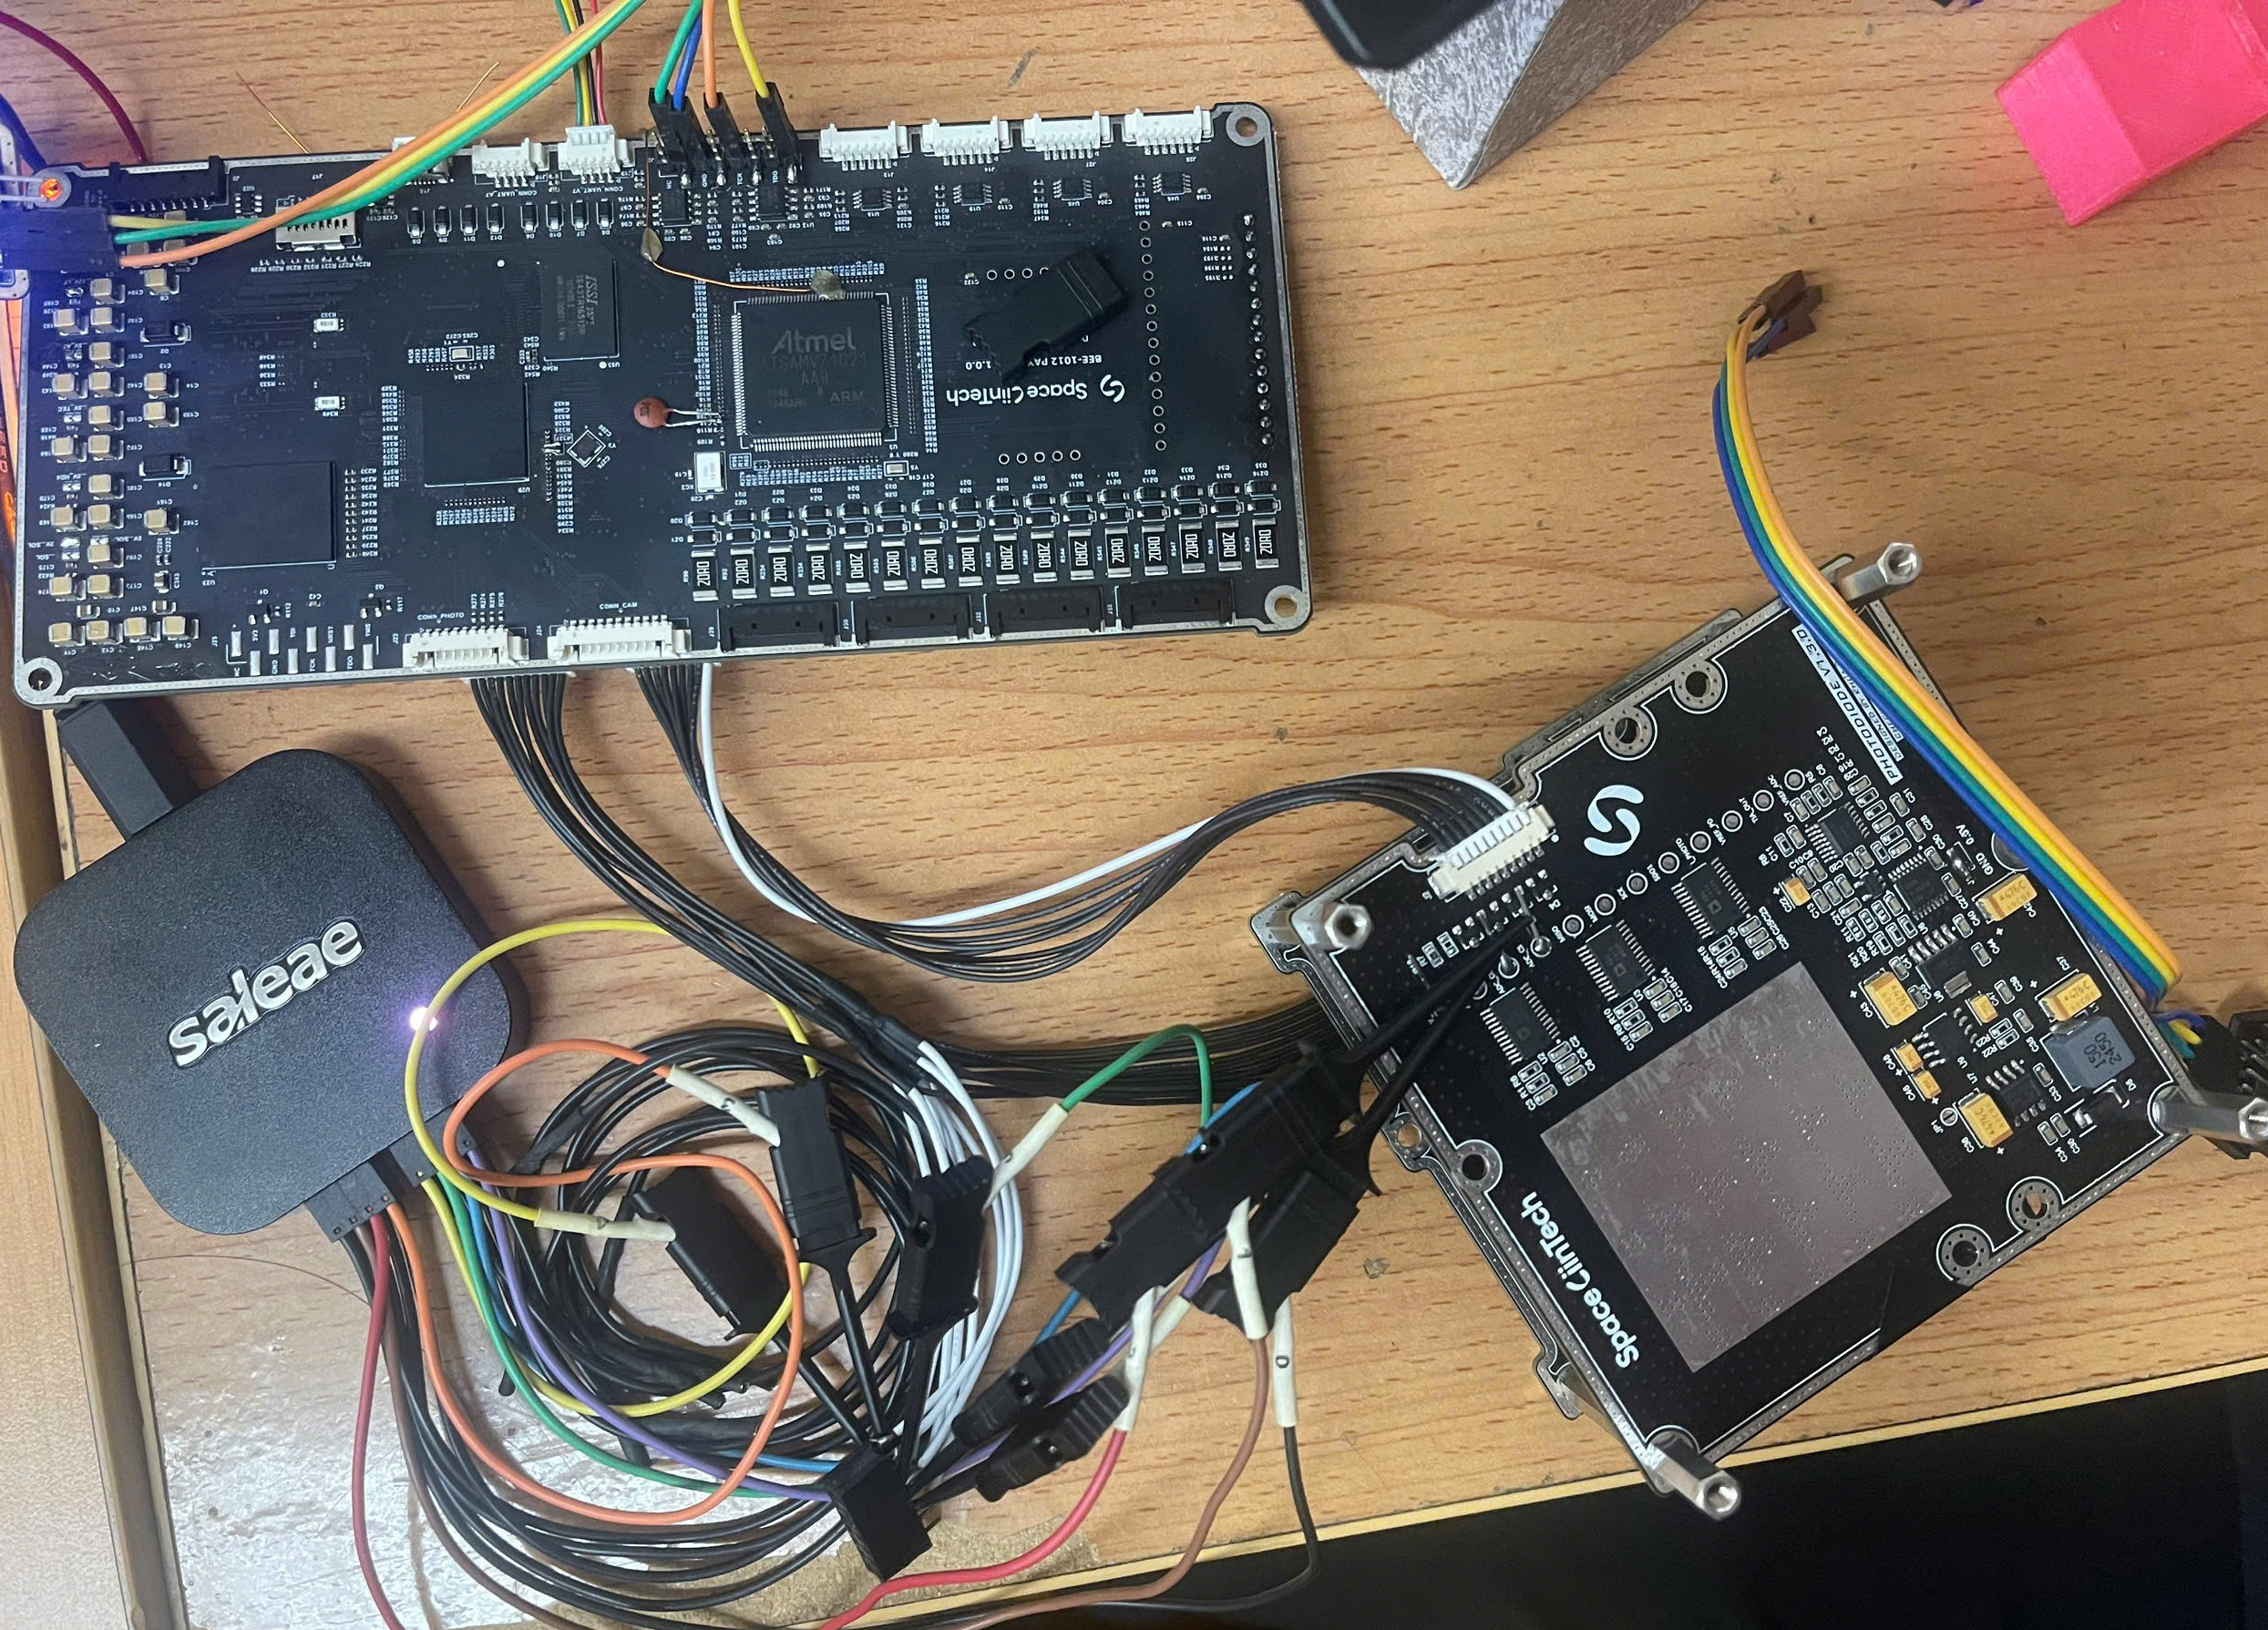
\includegraphics[width=0.9\textwidth]{picture/ket-qua/stack-up-board.jpg}
    \caption{Phần cứng thực tế các board chức năng của mô đun thí nghiệm}
    \label{fig:ket-qua-stack-up-board}
\end{figure}

Hình~\ref{fig:ket-qua-stack-up-board} thể hiện mô hình tích hợp thực tế của hệ thống trong quá trình kiểm thử. Các board được kết nối thông qua cáp tín hiệu và đầu nối mở rộng, trong đó board điều khiển trung tâm đảm nhiệm vai trò điều phối, còn các board ngoại vi phục vụ đo lường và điều khiển thí nghiệm. Việc tích hợp thành công ở mức phần cứng cho phép tiếp tục kiểm thử các chức năng phần mềm như giao tiếp UART, điều khiển laser, đọc dữ liệu cảm biến và cập nhật firmware.

Kết quả này cho thấy thiết kế cơ khí và bố trí đầu nối đã hỗ trợ được quá trình lắp ráp, tháo rời và kiểm thử từng phần. Đây là yêu cầu quan trọng đối với một mô đun thí nghiệm đa năng, vì hệ thống cần có khả năng thay đổi hoặc bổ sung board chức năng tùy theo cấu hình thí nghiệm.

\section{Kết quả xây dựng giao diện giám sát và điều khiển}
\label{sec:ket-qua-giao-dien}

Giao diện điều khiển trung tâm được xây dựng nhằm hỗ trợ quá trình vận hành, quan sát trạng thái và kiểm thử các chức năng của mô đun cấu hình thí nghiệm. Giao diện cho phép người dùng theo dõi dữ liệu cảm biến, quan sát đáp ứng điều khiển nhiệt độ, cấu hình profile vận hành, điều khiển cụm laser và quản lý kết nối UART với hệ thống phần cứng.

\begin{figure}[H]
    \centering
    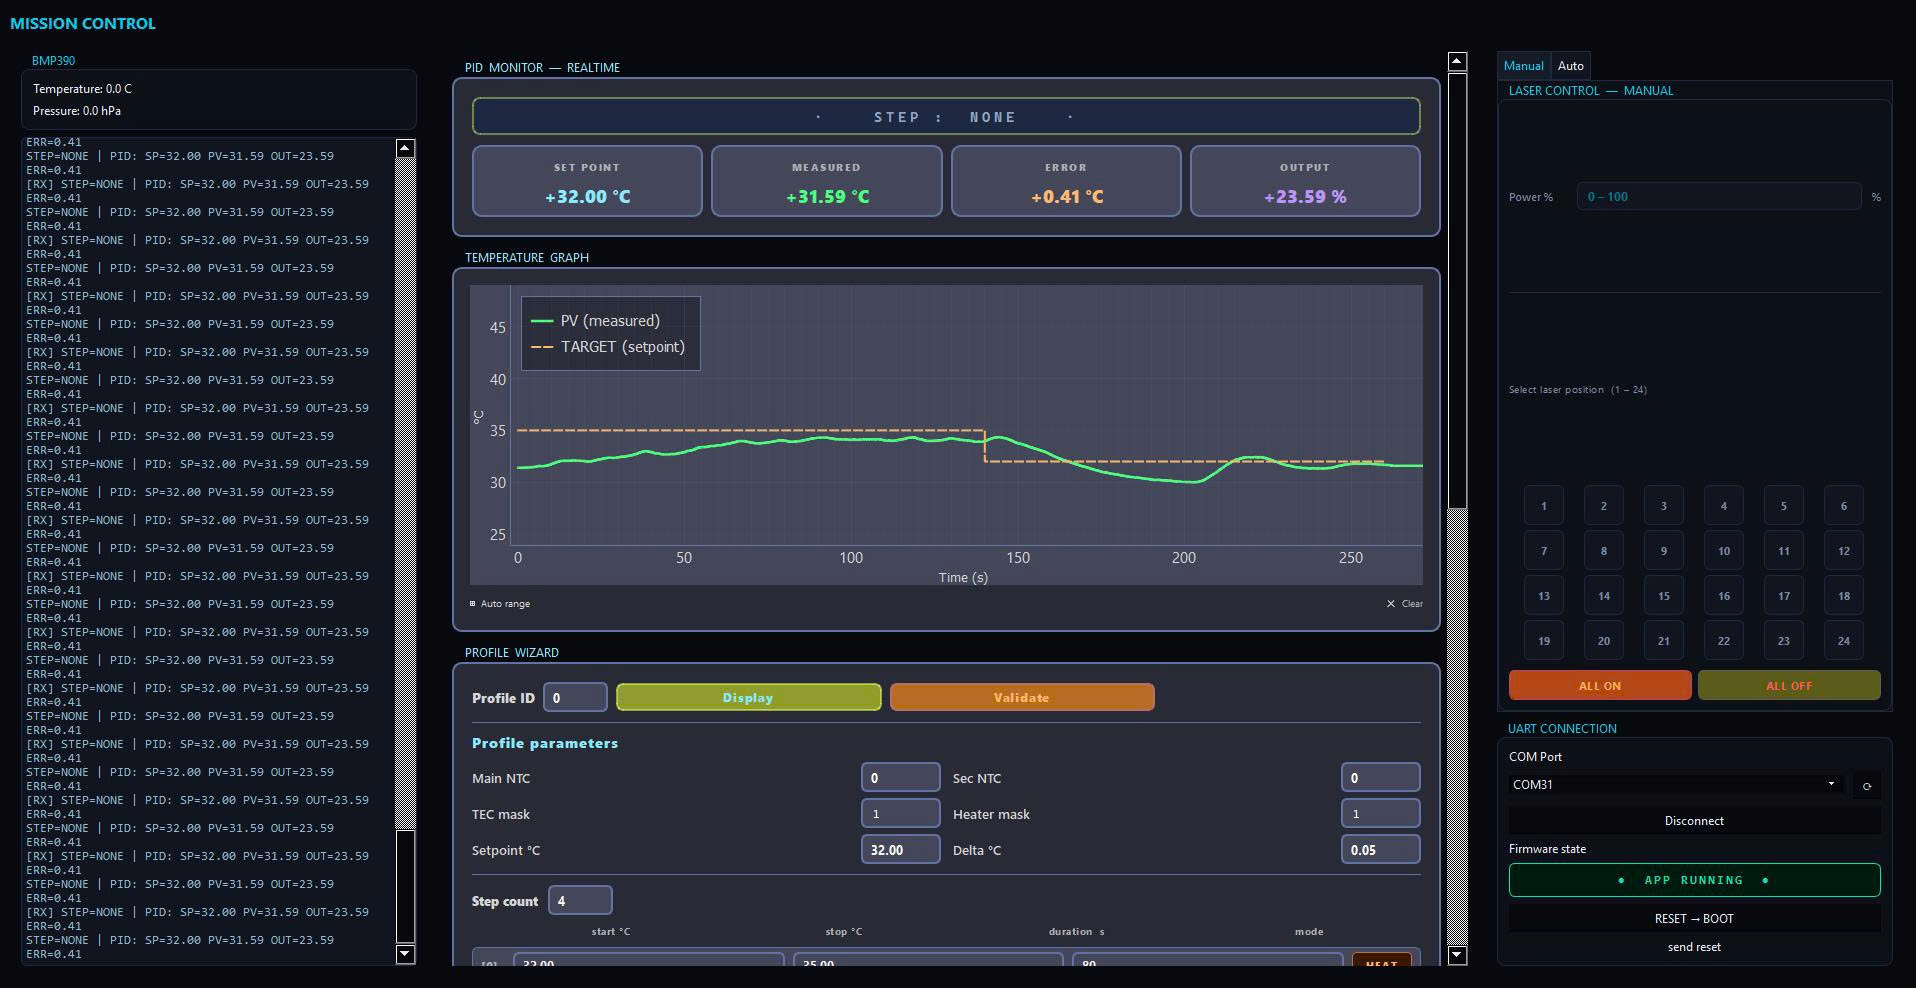
\includegraphics[width=1\textwidth]{picture/ket-qua/ui-control.jpg}
    \caption{Giao diện Mission Control dùng để giám sát và điều khiển hệ thống}
    \label{fig:ket-qua-ui-control}
\end{figure}

Hình~\ref{fig:ket-qua-ui-control} thể hiện giao diện Mission Control sau khi kết nối với hệ thống. Phần bên trái hiển thị dữ liệu nhận được từ UART, bao gồm trạng thái bước điều khiển, giá trị đặt, giá trị đo, sai số và ngõ ra điều khiển. Việc hiển thị liên tục các gói dữ liệu giúp người vận hành kiểm tra được luồng truyền thông giữa máy tính và phần cứng, đồng thời hỗ trợ phát hiện lỗi trong quá trình thử nghiệm.

Khu vực trung tâm của giao diện hiển thị các thông số chính của bộ điều khiển PID theo thời gian thực. Các giá trị gồm nhiệt độ đặt \textit{Set point}, nhiệt độ đo \textit{Measured}, sai số \textit{Error} và phần trăm ngõ ra \textit{Output}. Trong kết quả thử nghiệm, hệ thống ghi nhận giá trị đặt khoảng 32,00\,$^\circ$C, giá trị đo khoảng 31,59\,$^\circ$C và sai số khoảng 0,41\,$^\circ$C. Sai số này cho thấy bộ điều khiển có khả năng đưa nhiệt độ tiến gần đến giá trị đặt và duy trì trong vùng làm việc mong muốn.

Đồ thị nhiệt độ trên giao diện cho phép quan sát trực quan đáp ứng của hệ thống theo thời gian. Đường \textit{PV} biểu diễn giá trị nhiệt độ đo được, trong khi đường \textit{Target} biểu diễn nhiệt độ mục tiêu. Khi giá trị đặt thay đổi, nhiệt độ đo có xu hướng bám theo giá trị mục tiêu và ổn định lại sau một khoảng thời gian quá độ. Điều này cho thấy luồng đọc cảm biến, tính toán điều khiển và phản hồi dữ liệu về giao diện đã hoạt động đúng theo thiết kế.

Bên cạnh chức năng giám sát nhiệt độ, giao diện cũng hỗ trợ cấu hình profile vận hành. Người dùng có thể nhập các tham số như cảm biến NTC chính, cảm biến NTC phụ, mặt nạ TEC, mặt nạ Heater, nhiệt độ đặt, sai số cho phép và số lượng bước trong profile. Các chức năng hiển thị và kiểm tra profile giúp giảm sai sót trước khi gửi cấu hình xuống hệ thống phần cứng.

\section{Kết quả điều khiển cụm laser}
\label{sec:ket-qua-laser}

Khối điều khiển laser trên giao diện được thiết kế để hỗ trợ hai chế độ vận hành: thủ công và tự động. Ở chế độ thủ công, người dùng có thể thiết lập công suất laser theo phần trăm và lựa chọn vị trí laser cần kích hoạt. Giao diện bố trí 24 vị trí laser tương ứng với các kênh điều khiển trong hệ thống, đồng thời cung cấp các lệnh bật toàn bộ và tắt toàn bộ để phục vụ quá trình kiểm thử nhanh.

Kết quả trên giao diện cho thấy các thành phần điều khiển laser đã được tích hợp vào cùng một môi trường vận hành với phần giám sát nhiệt độ và kết nối UART. Cách tổ chức này giúp người vận hành có thể đồng thời theo dõi trạng thái hệ thống, điều khiển nguồn phát quang và quan sát dữ liệu phản hồi mà không cần sử dụng nhiều công cụ rời rạc.

Việc tách riêng chế độ \textit{Manual} và \textit{Auto} cũng tạo cơ sở cho quá trình phát triển các kịch bản thí nghiệm tự động. Trong giai đoạn kiểm thử, chế độ thủ công được sử dụng để kiểm tra từng kênh laser, kiểm tra đáp ứng của mạch công suất và xác nhận khả năng phát lệnh từ giao diện xuống phần cứng.

\begin{figure}[H]
    \centering
    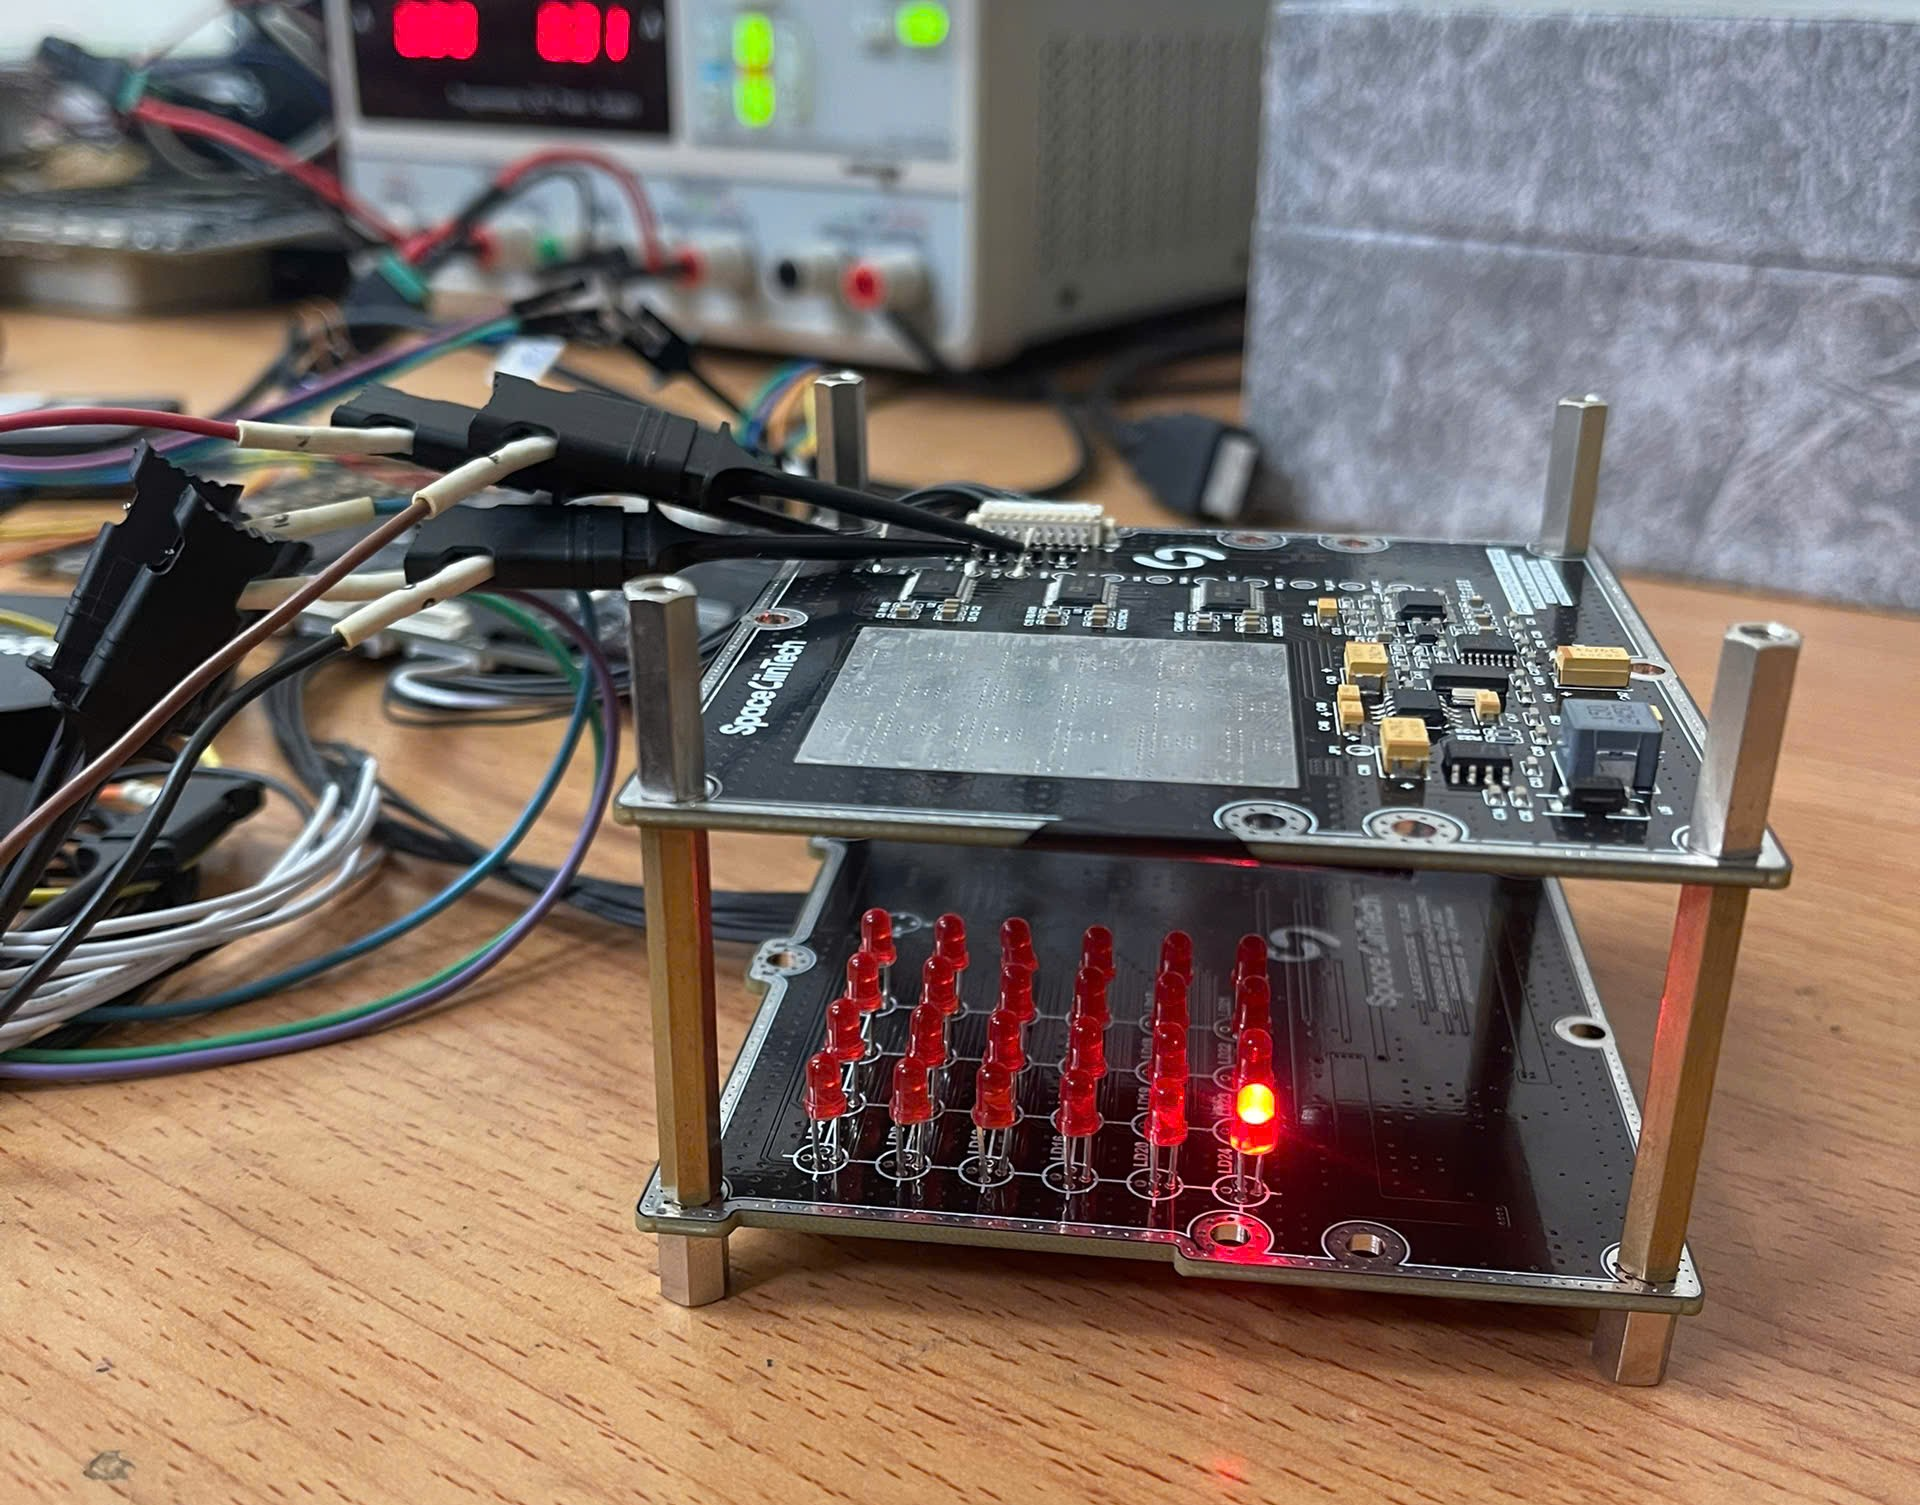
\includegraphics[width=0.75\textwidth]{picture/ket-qua/demo-laser.jpg}
    \caption{Kết quả kiểm thử điều khiển kênh laser trên phần cứng thực tế}
    \label{fig:ket-qua-demo-laser}
\end{figure}

Hình~\ref{fig:ket-qua-demo-laser} thể hiện kết quả kiểm thử điều khiển laser trên phần cứng thực tế. Một kênh laser được kích hoạt, trong khi các kênh còn lại ở trạng thái tắt. Kết quả này xác nhận lệnh điều khiển từ hệ thống có thể tác động đến đúng kênh đầu ra, đồng thời cho phép quan sát trực tiếp trạng thái hoạt động của cụm laser trong quá trình kiểm thử.

\section{Kết quả kết nối UART và trạng thái firmware}
\label{sec:ket-qua-uart-firmware}

Giao diện Mission Control hỗ trợ lựa chọn cổng COM, kết nối hoặc ngắt kết nối UART và hiển thị trạng thái firmware của hệ thống. Trong kết quả thử nghiệm, hệ thống được kết nối thông qua cổng COM31 và trạng thái firmware hiển thị là \texttt{APP RUNNING}. Điều này cho thấy ứng dụng chính trên MCU đã được nạp và đang thực thi.

Chức năng \textit{RESET BOOT} và lệnh gửi reset cho phép người vận hành chuyển hệ thống từ chế độ chạy ứng dụng sang chế độ Bootloader khi cần cập nhật firmware. Nhờ đó, quá trình kiểm thử phần mềm có thể được thực hiện thuận tiện hơn, đặc biệt trong các giai đoạn cần nạp nhiều phiên bản firmware để hiệu chỉnh thuật toán điều khiển hoặc kiểm tra giao tiếp.

\section{Kết quả thử nghiệm Bootloader thông qua MPU}
\label{sec:ket-qua-bootloader}

Chức năng Bootloader được kiểm thử nhằm đánh giá khả năng cập nhật firmware cho MCU thông qua MPU. Trong cấu hình này, MPU đóng vai trò là thiết bị trung gian, nhận lệnh từ người vận hành và truyền dữ liệu firmware xuống MCU bằng giao thức xTP. MCU sau đó xử lý các khung dữ liệu, ghi vào bộ nhớ Flash, kiểm tra tính toàn vẹn và chuyển sang chạy ứng dụng khi quá trình cập nhật hoàn tất.

\begin{figure}[H]
    \centering
    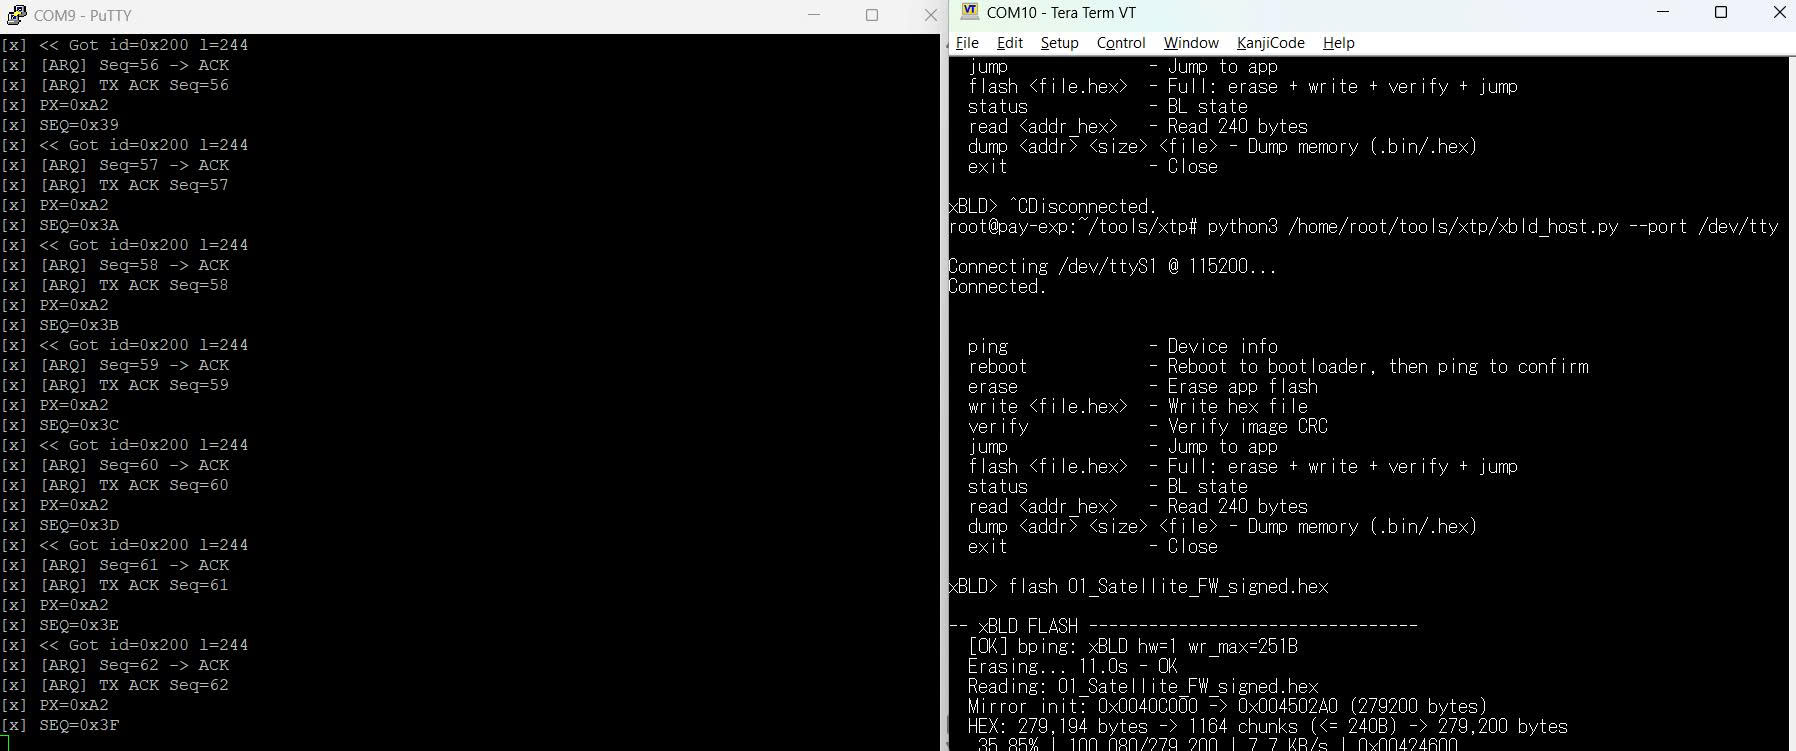
\includegraphics[width=1\textwidth]{picture/ket-qua/bootloader-mpu.jpg}
    \caption{Kết quả thử nghiệm cập nhật firmware Bootloader thông qua MPU}
    \label{fig:ket-qua-bootloader-mpu}
\end{figure}

Hình~\ref{fig:ket-qua-bootloader-mpu} trình bày quá trình thử nghiệm Bootloader. Cửa sổ bên phải thể hiện giao diện dòng lệnh trên MPU, trong đó công cụ \texttt{xbld\_host.py} được sử dụng để kết nối đến MCU thông qua cổng UART nội bộ. Sau khi kết nối thành công, người vận hành có thể sử dụng các lệnh như \texttt{ping}, \texttt{reboot}, \texttt{erase}, \texttt{write}, \texttt{verify}, \texttt{jump} và \texttt{flash}.

Khi thực hiện lệnh \texttt{flash} với tệp firmware, chương trình tiến hành xóa vùng nhớ ứng dụng, đọc dữ liệu từ tệp hex, chia dữ liệu thành các khối nhỏ và truyền xuống MCU. Kết quả hiển thị cho thấy hệ thống bắt đầu quá trình ghi firmware với kích thước dữ liệu khoảng 279.200 bytes. Điều này xác nhận luồng truyền firmware từ MPU xuống MCU đã được kích hoạt đúng.

Cửa sổ bên trái thể hiện quá trình xử lý gói tin ở phía nhận. Các dòng log có dạng \texttt{Got id=0x200}, \texttt{Seq} và \texttt{ACK} cho thấy MCU nhận được các khung dữ liệu và gửi phản hồi xác nhận sau từng gói. Cơ chế đánh số thứ tự gói và phản hồi ACK giúp kiểm soát quá trình truyền, hạn chế lỗi mất gói hoặc sai thứ tự trong quá trình cập nhật firmware.

Kết quả thử nghiệm chứng minh Bootloader đã đáp ứng các yêu cầu chính:

\begin{itemize}
    \item Có thể kết nối từ MPU đến MCU thông qua UART.
    \item Có thể nhận lệnh điều khiển Bootloader từ công cụ phía host.
    \item Có thể truyền firmware theo từng khối dữ liệu nhỏ.
    \item Có cơ chế phản hồi ACK theo từng gói để kiểm soát lỗi truyền.
    \item Có khả năng thực hiện chuỗi thao tác xóa, ghi, kiểm tra và chuyển sang ứng dụng.
\end{itemize}

Như vậy, chức năng cập nhật firmware từ xa ở mức hệ thống đã được kiểm chứng. Đây là một kết quả quan trọng vì mô đun cấu hình thí nghiệm cần có khả năng bảo trì và cập nhật phần mềm sau khi đã tích hợp vào hệ thống lớn hơn.

\section{Đánh giá kết quả đạt được}
\label{sec:danh-gia-ket-qua}

Từ các kết quả thử nghiệm, hệ thống đã hoàn thành các chức năng cốt lõi đặt ra trong phạm vi luận văn. Về phần cứng, kiến trúc mô đun gồm các khối xử lý, giao tiếp, điều khiển ngoại vi và nguồn đã tạo nền tảng để triển khai các thí nghiệm khác nhau. Về phần mềm, hệ thống đã có giao diện giám sát, firmware điều khiển thời gian thực và Bootloader phục vụ cập nhật chương trình.

Giao diện Mission Control cho phép vận hành hệ thống ở mức tích hợp, trong đó người dùng có thể quan sát dữ liệu, cấu hình profile nhiệt độ, điều khiển laser và quản lý trạng thái firmware. Kết quả đồ thị nhiệt độ cho thấy luồng điều khiển PID đã hoạt động và có khả năng bám theo giá trị đặt. Kết quả thử nghiệm Bootloader cho thấy quá trình truyền firmware qua MPU có phản hồi ACK và có thể thực hiện theo chuỗi thao tác đã thiết kế.

Tuy nhiên, các kết quả hiện tại chủ yếu tập trung vào kiểm chứng chức năng và luồng vận hành. Một số đánh giá định lượng chuyên sâu như độ ổn định nhiệt trong thời gian dài, sai số giữa nhiều cảm biến, độ lặp lại của từng kênh laser, tốc độ cập nhật firmware trong nhiều điều kiện truyền thông và khả năng chịu lỗi khi mất kết nối vẫn cần được tiếp tục khảo sát trong các giai đoạn phát triển sau.
